\documentclass[border=8pt]{standalone}
% shared preamble for case-study figures
\usepackage{tikz}
\usepackage{helvet}
\renewcommand{\familydefault}{\sfdefault}
\usetikzlibrary{arrows.meta, positioning}
\definecolor{boxfill}{RGB}{223,233,242}
\definecolor{boxborder}{RGB}{74,122,155}
\definecolor{termfill}{RGB}{28,61,82}
\definecolor{failfill}{RGB}{248,224,220}
\definecolor{failborder}{RGB}{178,55,42}
\definecolor{qgray}{RGB}{120,120,120}
\tikzset{
  box/.style={rectangle, rounded corners=3pt, draw=boxborder, line width=1pt,
              fill=boxfill, text width=74mm, align=center, inner sep=6pt, font=\small},
  failbox/.style={rectangle, rounded corners=3pt, draw=failborder, line width=1pt,
              fill=failfill, text width=74mm, align=center, inner sep=6pt, font=\small},
  term/.style={rectangle, rounded corners=3pt, draw=termfill, line width=1pt,
               fill=termfill, text=white, text width=74mm, align=center, inner sep=7pt, font=\small},
  failterm/.style={rectangle, rounded corners=3pt, draw=failborder, line width=1pt,
               fill=failborder, text=white, text width=74mm, align=center, inner sep=7pt, font=\small},
  hdr/.style={text width=80mm, align=center, font=\small},
  arr/.style={-{Stealth[length=3mm]}, line width=1pt, draw=boxborder}
}
\newcommand{\gate}[5]{\textbf{#1}\hfill\textcolor{qgray}{\textit{#2}}\\[2pt] P~=~#3\quad threshold~=~#4\\[2pt] \textbf{Result $\rightarrow$ #5}}

\begin{document}
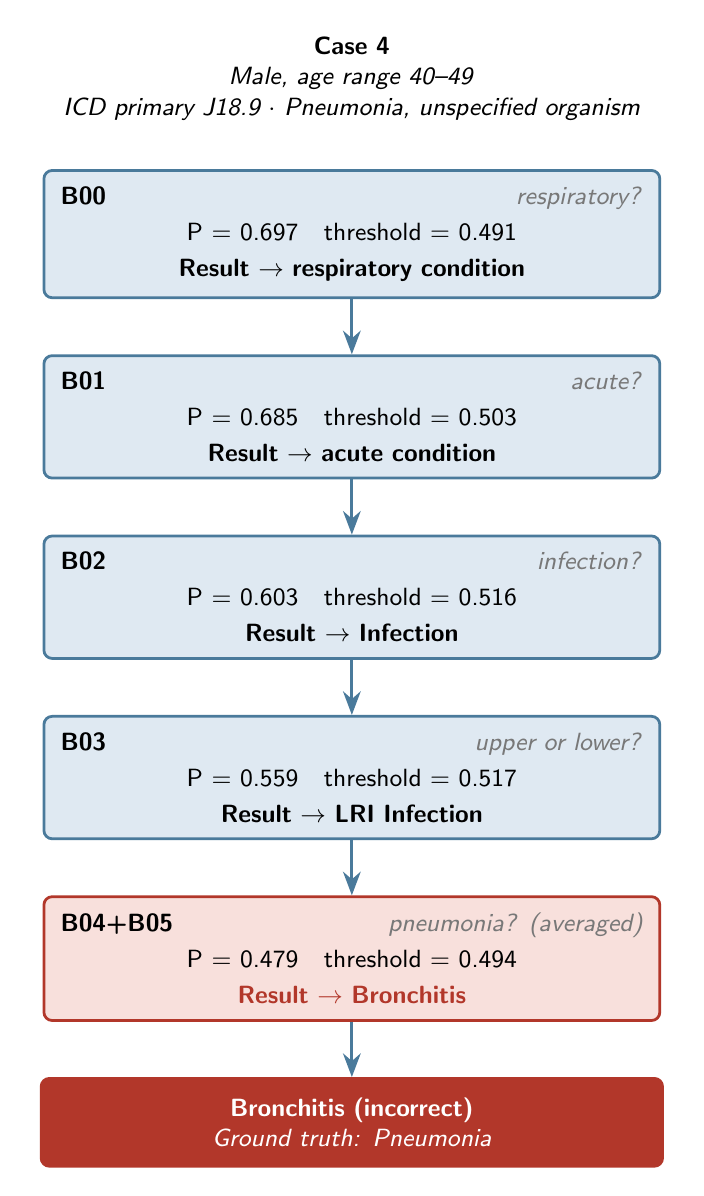
\begin{tikzpicture}[node distance=7mm]
\node[hdr] (h) {\textbf{Case 4}\\ \textit{Male, age range 40--49}\\ \textit{ICD primary J18.9 $\cdot$ Pneumonia, unspecified organism}};
\node[box, below=5mm of h] (b0) {\gate{B00}{respiratory?}{0.697}{0.491}{respiratory condition}};
\node[box, below=of b0] (b1) {\gate{B01}{acute?}{0.685}{0.503}{acute condition}};
\node[box, below=of b1] (b2) {\gate{B02}{infection?}{0.603}{0.516}{Infection}};
\node[box, below=of b2] (b3) {\gate{B03}{upper or lower?}{0.559}{0.517}{LRI Infection}};
\node[failbox, below=of b3] (b4) {\textbf{B04+B05}\hfill\textcolor{qgray}{\textit{pneumonia? (averaged)}}\\[2pt] P~=~0.479\quad threshold~=~0.494\\[2pt] \textbf{\textcolor{failborder}{Result $\rightarrow$ Bronchitis}}};
\node[failterm, below=of b4] (t) {\textbf{Bronchitis (incorrect)}\\ \textit{Ground truth: Pneumonia}};
\draw[arr] (b0)--(b1); \draw[arr] (b1)--(b2); \draw[arr] (b2)--(b3); \draw[arr] (b3)--(b4); \draw[arr] (b4)--(t);
\end{tikzpicture}
\end{document}
